\documentclass[a4paper]{report}

\usepackage{amsmath}
\usepackage{amsfonts}
\usepackage{graphicx}

\begin{document}

\section{Kinematics}
Kinematics is the science that studies the geometry of motion. It is restricted
to a purely geometrical description of motion by means of position, orientation
and their time derivatives.

Kinematic models are also fundamental to study the dynamics of the robots and
also to design controllers.

In robotics, kinematics helps to answer two questions:
\begin{itemize}
    \item{} Given a set of values for the different joint parameters (elbows,
        knees, etc.) where would the end effector (hand, foot, etc.) be located?
        This is known as forward kinematics.
    \item{} To position the end effector in a particular place for instance to
        reach the door's knob or to place the foot in the right spot not fall, how
        should the joint parameters be set? This is known as inverse kinematics.
\end{itemize}

The second problem is more interesting but it is also more complicated as multiple
solutions may exist for the same problem <reference>.


\section{Absolute and relative coordinate systems}
The study of kinematics begins by defining a global coordinate system, such
coordinate system will serve to describe the position of the robot and its
parts, as well as the position of all the other objects of interest in world.
This is known as the world coordinate system $\Sigma_W$, its origin can be
fixed anywhere in the world. When the position of an object is given in
world coordinates it is common to refer to this position as the absolute
position, mathematically coordinates are represented by three dimensional vectors:
\begin{equation}
    \boldsymbol{p} = \begin{bmatrix}
        p_x\\
        p_y\\
        p_x\\
    \end{bmatrix}
\end{equation}

From time to time it is also convenient to have additional coordinate systems to
describe where things are located with respect to other objects in the world, for
example for a humanoid robot it may be useful to know where the door's knob is
located with respect to its hand or where the end of its arm is located with
respect to its elbow. In both examples the coordinate systems are attached to
a particular object (the hand, the elbow) and they move with that particular
object, these kind of coordinate systems are known as local coordinate systems.


\section{Homogeneous Transformations}
The use of multiple coordinate systems introduces a new problem, the same point
can be represented in multiple coordinate systems, a mechanism to transform the
coordinates of an object between coordinate systems is required. As shown by
<reference> such transformation can be performed with homogeneous transformation
matrices, given a point $h$ with coordinates $^{b}\boldsymbol{p}_{h}$ in
a local coordinate system $\Sigma_b$ which has its $x_b$, $y_b$ and $z_b$ axis
rotated $\phi$, $\theta$ and $\psi$ degrees with respect to the $x_a$, $y_a$
and $z_a$ axis of another local coordinate system $\Sigma_{a}$, the coordinates
$^{a}\boldsymbol{p}_{h}$ of the point $h$ in $\Sigma_b$ is given by:

\begin{equation}
    \begin{bmatrix} ^{a}\boldsymbol{p}_{h} \\ 1 \end{bmatrix} = \,
        ^{a}\boldsymbol{T}_{b}
        \begin{bmatrix}
            ^{b}\boldsymbol{p}_{h} \\ 1
        \end{bmatrix} =
        \begin{bmatrix}
            ^{a}\boldsymbol{R}_{b} & ^{a}\boldsymbol{p}_{b} \\
            0 & 0 & 0 & 1
        \end{bmatrix}
        \begin{bmatrix}
            \boldsymbol{^{b}p_{h}} \\
            1
        \end{bmatrix}
\end{equation}

Where:
\begin{itemize}
    \item{} $^{a}\boldsymbol{T}_{b}$ is a $4x4$ known as the homogeneous transformation matrix.
    \item{} $^{a}\boldsymbol{R}_{b}$ the rotation matrix, more on this below.
    \item{} $^{a}\boldsymbol{p}_{b}$ is the origin of $\Sigma_{b}$ viewed from $\Sigma_{a}$.
\end{itemize}

It's important to note that the homogeneous transformation matrix takes into
account both the rotational and the translational transformation.


\subsection{Rotation Matrix}\label{sub:rotation_matrix}
The rotation matrix can be seen in two different ways:
\begin{itemize}
    \item{} As a pure mathematical operator that rotates vectors <reference>
    \item{} As a matrix that represents the attitude of a local coordinate space
        and is defined as $\boldsymbol{R} = [e_x, e_y, e_z]$ as shown in figure
        \ref{fig:rotation_matrix}, where $e_x$, $e_y$ and $e_z$ are unit vectors
        in the direction of the axis $x$, $y$ and $z$ of the local coordinate
        system.
\end{itemize}

\begin{figure}[htb!]
\begin{center}
    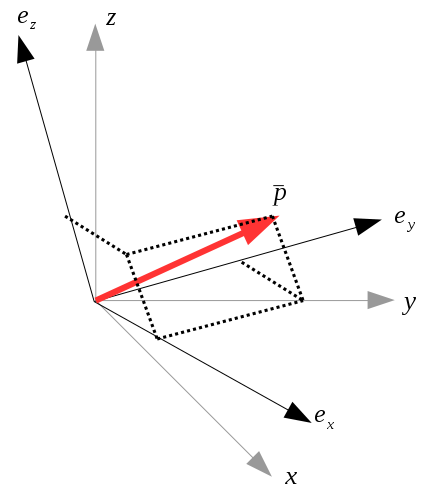
\includegraphics[width=0.5\textwidth]{./resources/rotation_matrix.png}
    \caption{Rotation matrix as the attitude of a coordinate system}
    \label{fig:rotation_matrix}
\end{center}
\end{figure}

The rotational matrix has another interesting property, from a linear algebra
point of view this matrix is orthogonal and it can be proved that <reference>:
\begin{equation}
    \boldsymbol{R}^{-1} = \boldsymbol{R}^{T}
\end{equation}

\subsection{Chain Rule}


\section{Angular Velocity}
By definition the speed of a point on a rigid body which is rotating about an
arbitrary axis in space is given by <reference>:
\begin{equation}
    \boldsymbol{v} = \boldsymbol{w} \times \boldsymbol{p} \label{eq:angularVelocity}
\end{equation}

Where $\boldsymbol{w}$ is the angular velocity vector and $\boldsymbol{p}$ is a
vector that represents a given point $p$ on the surface of the rigid body. The
geometrical meaning of equation \eqref{eq:angularVelocity} is given in figure
\ref{fig:rotation_velocity}.

\begin{figure}[htb!]
\begin{center}
    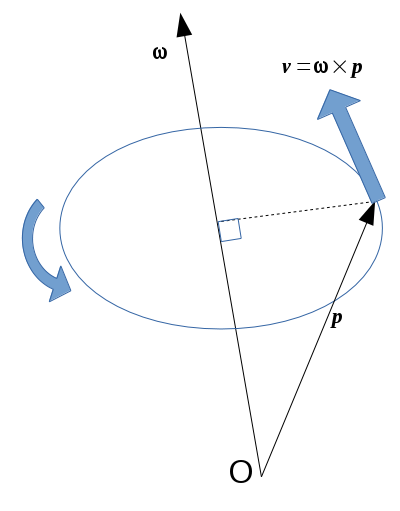
\includegraphics[width=0.5\textwidth]{./resources/rotational_speed.png}
    \caption{Angular velocity}
    \label{fig:rotation_velocity}
\end{center}
\end{figure}


Just as position vectors, velocity vectors can also be rotated:
\begin{equation}
\begin{split}
    \boldsymbol{v}\,' = \boldsymbol{R} \boldsymbol{v} \\
    \boldsymbol{p}\,' = \boldsymbol{R} \boldsymbol{p} \\
    \boldsymbol{w}\,' = \boldsymbol{R} \boldsymbol{w}
\end{split}
\end{equation}

Thus:
\begin{equation}
\begin{split}
    \boldsymbol{v}\,' = \boldsymbol{w}\,' \times \boldsymbol{p}\,' \\
    \boldsymbol{R}\boldsymbol{v} = \boldsymbol{R} \boldsymbol{w} \times \boldsymbol{R} \boldsymbol{p}
\end{split}
\end{equation}

A rotation matrix can be interpreted as a mathematical operator that rotates vectors
(see section \ref{sub:rotation_matrix}), and the position of a vector $\boldsymbol{p}$
after the rotation is given by:

\begin{equation}
    \boldsymbol{p} = \boldsymbol{R} \bar{\boldsymbol{p}} \label{eq:rotateVector}
\end{equation}

Where $\bar{\boldsymbol{p}}$ is the original position vector before the rotation,
taking the derivative of this expression with respect to time:

\begin{equation}
\begin{split}
    \frac{d}{dt}\big( \boldsymbol{p} = \boldsymbol{R} \bar{\boldsymbol{p}} \big) \\
    \boldsymbol{v} = \dot{\boldsymbol{p}}\ = \boldsymbol{\dot{R}} \bar{\boldsymbol{p}} + \boldsymbol{R} \dot{\bar{\boldsymbol{p}}}
\end{split}
\end{equation}

But $\bar{\boldsymbol{p}}$ is constant, so the previous equation becomes:

\begin{equation}
    \boldsymbol{v} = \boldsymbol{\dot{R}} \bar{\boldsymbol{p}} \label{eq:positionDerivative}
\end{equation}

From equation \eqref{eq:rotateVector}:
\begin{equation}
\begin{split}
    \bar{\boldsymbol{p}} = \boldsymbol{R^{-1}} \boldsymbol{p} = \boldsymbol{R^{T}} \boldsymbol{p}
\end{split}
\end{equation}

Substituting this result in equation \eqref{eq:positionDerivative}:
\begin{equation}
\begin{split}
    \boldsymbol{v} = \boldsymbol{\dot{R}} \bar{\boldsymbol{p}} = \boldsymbol{\dot{R}} \boldsymbol{R^{T}} \boldsymbol{p}
\end{split}
\end{equation}

This equation provides an alternative method to calculate, the speed of a point $p$
on a rigid body which is rotating about an arbitrary axis in space, comparing it
against the definition given before (equation \eqref{eq:angularVelocity}):
\begin{equation}
\begin{split}
    \boldsymbol{v} = \boldsymbol{w} \times \boldsymbol{p} = \boldsymbol{\dot{R}} \boldsymbol{R^{T}} \boldsymbol{p} \label{eq:angularVelocityAlternative}
\end{split}
\end{equation}

The cross product can also be written as the product of skew-symmetric matrix and a vector <reference>:

\begin{equation}
    \boldsymbol{w} \times \boldsymbol{p} = \hat{\boldsymbol{w}} \boldsymbol{p} =
    \begin{bmatrix}
        0 & -w_z & w_y \\
        w_z & 0 & -w_x \\
        -w_y & w_x & 0
    \end{bmatrix} \boldsymbol{p}
\end{equation}

With this in mind equation \eqref{eq:angularVelocityAlternative} can be rewritten as:
\begin{equation}
\begin{split}
    \boldsymbol{v} = \hat{\boldsymbol{w}} \boldsymbol{p} = \boldsymbol{\dot{R}} \boldsymbol{R^{T}} \boldsymbol{p}
\end{split}
\end{equation}

Therefore:
\begin{equation}
    \hat{\boldsymbol{w}} = \boldsymbol{\dot{R}} \boldsymbol{R^{T}} \label{eq:hatAngularVelocity}
\end{equation}

Following the convention introduced by \ref{kajita} to refer to 3 dimensional vectors
taken from Skew Symmetric Matrices as the $\vee$ "wedge" operation, and making a Skew
Symmetric matrix from a 3 dimensional vector will be referred to as taking the
$\wedge$ "hat" operation as follows:

\begin{equation}
\begin{split}
    \begin{bmatrix}
        0 & -w_z & w_y \\
        w_z & 0 & -w_x \\
        -w_y & w_x & 0
    \end{bmatrix}^{\vee} = \begin{bmatrix} w_x \\ w_y \\ w_x\end{bmatrix} \\
    \begin{bmatrix} w_x \\ w_y \\ w_x\end{bmatrix}^{\wedge} =
    \begin{bmatrix}
        0 & -w_z & w_y \\
        w_z & 0 & -w_x \\
        -w_y & w_x & 0
    \end{bmatrix}
\end{split}
\end{equation}

Finally the angular Velocity is given by:
\begin{equation}
    \boldsymbol{w} = (\boldsymbol{\dot{R}} \boldsymbol{R^{T}})^{\vee}
\end{equation}

This equation allows to compute the angular speed directly from the rotation matrix.

\section{Velocity in Three Dimensional Space}

\subsection{Single Object}
In general an object in a three dimensional space can be subject to both translational
and rotational motion, to study its kinematics a global coordinate system $\Sigma_W$
should be defined and a local coordinate system attached to the given object to
describe its attitude, this is shown in figure \ref{fig:single_object_velocity}.

\begin{figure}[htb!]
\begin{center}
    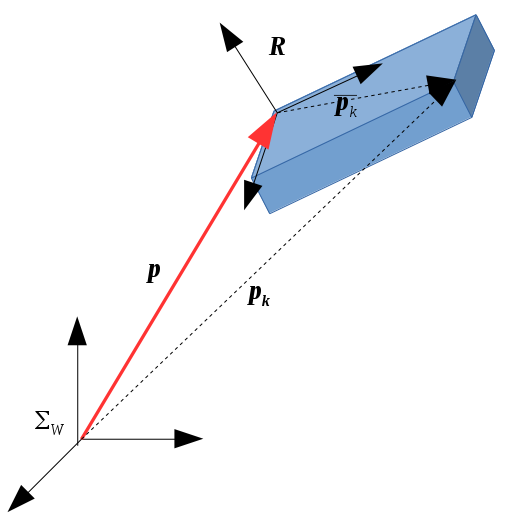
\includegraphics[width=0.5\textwidth]{./resources/single_object_velocity.png}
    \caption{Position and attitude for an object in space}
    \label{fig:single_object_velocity}
\end{center}
\end{figure}

The position of the point $p_k$ in the global coordinate system is given by:

\begin{equation*}
    \boldsymbol{p}_k = \boldsymbol{p} + \boldsymbol{R} \bar{\boldsymbol{p}}_k
\end{equation*}

Taking the time derivative of this equation:
\begin{equation}
\begin{split}
    \frac{d}{dt}(\boldsymbol{p}_k = \boldsymbol{p} + \boldsymbol{R} \bar{\boldsymbol{p}}_k) \\
    \boldsymbol{\dot{p}}_k = \boldsymbol{\dot{p}} + \boldsymbol{\dot{R}} \bar{\boldsymbol{p}}_k
\end{split}
\end{equation}

From \eqref{eq:hatAngularVelocity} $\dot{\boldsymbol{R}} = \boldsymbol{\hat{w}}\boldsymbol{R}$,
substituting this result in the previous expression:
\begin{equation}
\begin{split}
    \boldsymbol{\dot{p}}_k = \boldsymbol{\dot{p}} + \hat{w}\boldsymbol{R} \bar{\boldsymbol{p}}_k \\
    \boldsymbol{\dot{p}}_k = \boldsymbol{\dot{p}} + \boldsymbol{w} \times (\boldsymbol{R} \bar{\boldsymbol{p}}_k) \label{eq:singleObjectVelocity}
\end{split}
\end{equation}

Making some additional definitions, equation \eqref{eq:singleObjectVelocity} can
be re-written as follows:
\begin{equation}
    \boldsymbol{v}_k = \boldsymbol{v} + \boldsymbol{w} \times (\boldsymbol{p}_k - \boldsymbol{p})
\end{equation}

Where:
\begin{itemize}
    \item $\boldsymbol{v}_k = \boldsymbol{\dot{p}}_k$
    \item $\boldsymbol{\dot{p}} = \boldsymbol{v}$
    \item $\boldsymbol{R} \bar{\boldsymbol{p}}_k = \boldsymbol{p}_k - \boldsymbol{p}$
        Remember that $\bar{\boldsymbol{p}}_k$ does not change with respect to the
        local coordinate system attached to the object (See figure \ref{fig:single_object_velocity}).
\end{itemize}

\subsection{Multiple Objects}
A similar analysis can be applied to obtain the linear velocity and the angular
velocity equations for a second object that moves in a three dimensional
space. As before a global coordinate system should been defined and local coordinate
systems attached to the objects being studied, then the homogeneous transformation
matrices for these objects should be calculated. As a concrete example, consider
the case

<reference> kajita derived
\begin{equation}
    \boldsymbol{v}_2 = \boldsymbol{v}_1 + \boldsymbol{R}_1  + \boldsymbol{w}_1 \times (\boldsymbol{p}_2 - \boldsymbol{p}_1)
\end{equation}


\end{document}
